\documentclass{article}
\usepackage{subfiles}
\usepackage{graphicx}
\usepackage{amsfonts}
\usepackage{amsmath}
\usepackage{amssymb}
\usepackage{amsthm}
\usepackage{enumitem}
\usepackage{caption}
\usepackage{tikz}
\usepackage{graphicx}
\usepackage{float}
\usepackage{url}
\usepackage{listofitems}
\usepackage{pgfplots}
\usepackage{hyperref}
\hypersetup{
    colorlinks=true,
    linktoc=all,
    linkcolor=blue,
}

\begin{document}

\newpage
    \subfile{Sources/titlepage}
\newpage

\newpage
    \tableofcontents
\newpage

\section{Graph Data Structure}
A \emph{graph} $G$ [\autoref{fig:example-graph}] is a non-linear data structure consisting of vertices and edges. The vertices are sometimes also referred to as nodes and the edges are arcs that connect any two nodes in the graph. Graphs are used to represent relationships between different entities and have applications in many fields including Computer Science, Physics, Biology, Chemistry, Optimization Theory and many more.

\begin{figure}[H]
    \centering
    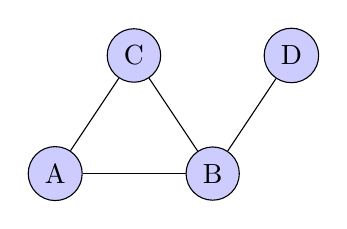
\begin{tikzpicture}
        % Define the vertices
        \node[circle, draw, fill=blue!20] (A) at (0,0) {A};
        \node[circle, draw, fill=blue!20] (B) at (2,0) {B};
        \node[circle, draw, fill=blue!20] (C) at (1,1.5) {C};
        \node[circle, draw, fill=blue!20] (D) at (3,1.5) {D};
        
        % Define the edges
        \draw (A) -- (B);
        \draw (A) -- (C);
        \draw (B) -- (C);
        \draw (B) -- (D);
    \end{tikzpicture}
    \caption{A simple graph}
    \label{fig:example-graph}
\end{figure}

\subsection{Formal Definition}
A graph is formally defined as a tuple $G = (V, E)$, where:
\begin{itemize}
    \item $V$ is a finite set of vertices (or nodes).
    \item $E$ is a set of edges, where each edge is an unordered pair of distinct vertices from $V$. Thus, $E \subseteq \{\{u, v\} \mid u, v \in V \text{ and } u \neq v\}$.
\end{itemize}

\subsection{Types of Graphs}
Graphs can be classified into various types based on their properties, including:
\begin{itemize}
    \item \textbf{Directed Graph} [\autoref{fig:directed-graph}]: A graph in which the edges have a direction, i.e., each edge is an ordered pair of vertices.
    
    \begin{figure}[H]
    \centering
    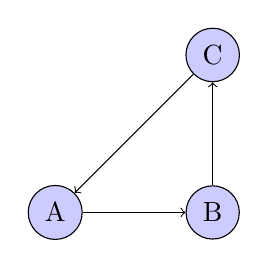
\begin{tikzpicture}
        % Vertices
        \node[circle, draw, fill=blue!20] (A) at (0,0) {A};
        \node[circle, draw, fill=blue!20] (B) at (2,0) {B};
        \node[circle, draw, fill=blue!20] (C) at (2,2) {C};
        
        % Directed edges
        \draw[->] (A) -- (B);
        \draw[->] (B) -- (C);
        \draw[->] (C) -- (A);
    \end{tikzpicture}
    \caption{Directed graph example.}
    \label{fig:directed-graph}
    \end{figure}

    \item \textbf{Undirected Graph} [\autoref{fig:undirected-graph}]: A graph in which the edges do not have a direction, i.e., each edge is an unordered pair of vertices.
    
    \begin{figure}[H]
    \centering
    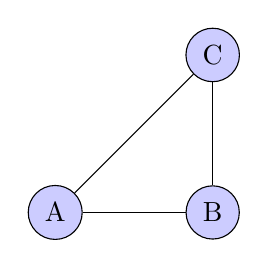
\begin{tikzpicture}
        % Vertices
        \node[circle, draw, fill=blue!20] (A) at (0,0) {A};
        \node[circle, draw, fill=blue!20] (B) at (2,0) {B};
        \node[circle, draw, fill=blue!20] (C) at (2,2) {C};
        
        % Undirected edges
        \draw (A) -- (B);
        \draw (B) -- (C);
        \draw (C) -- (A);
    \end{tikzpicture}
    \caption{Undirected graph example.}
    \label{fig:undirected-graph}
    \end{figure}
    
    \item \textbf{Weighted Graph} [\autoref{fig:weighted-graph}]: A graph in which a weight (or cost) is associated with each edge.
    
    \begin{figure}[H]
    \centering
    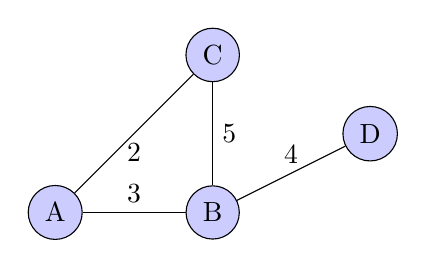
\begin{tikzpicture}
        % Vertices
        \node[circle, draw, fill=blue!20] (A) at (0,0) {A};
        \node[circle, draw, fill=blue!20] (B) at (2,0) {B};
        \node[circle, draw, fill=blue!20] (C) at (2,2) {C};
        \node[circle, draw, fill=blue!20] (D) at (4,1) {D};
        
        % Edges with weights
        \draw (A) -- node[above] {3} (B);
        \draw (B) -- node[right] {5} (C);
        \draw (C) -- node[below] {2} (A);
        \draw (B) -- node[above] {4} (D);
    \end{tikzpicture}
    \caption{Weighted graph example.}
    \label{fig:weighted-graph}
    \end{figure}
    
    \item \textbf{Simple Graph} [\autoref{fig:simple-graph}]: A graph with no loops (edges connecting a vertex to itself) and no multiple edges (more than one edge connecting the same pair of vertices).
    
    \begin{figure}[H]
    \centering
    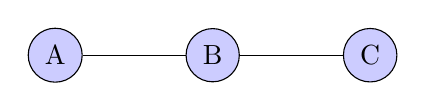
\begin{tikzpicture}
        % Vertices in a straight line
        \node[circle, draw, fill=blue!20] (A) at (0,0) {A};
        \node[circle, draw, fill=blue!20] (B) at (2,0) {B};
        \node[circle, draw, fill=blue!20] (C) at (4,0) {C};
        
        % Edges
        \draw (A) -- (B);
        \draw (B) -- (C);
    \end{tikzpicture}
    \caption{Simple graph example.}
    \label{fig:simple-graph}
    \end{figure}
    
    \item \textbf{Complete Graph} [\autoref{fig:complete-graph}]: A graph in which there is exactly one edge between each pair of distinct vertices.
    
    \begin{figure}[H]
    \centering
    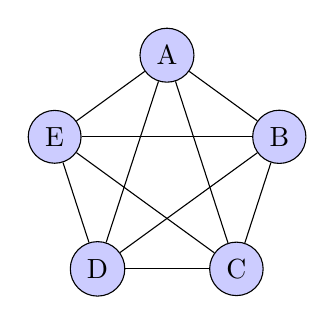
\begin{tikzpicture}
        % Vertices
        \node[circle, draw, fill=blue!20] (A) at (90:1.5cm) {A};
        \node[circle, draw, fill=blue!20] (B) at (18:1.5cm) {B};
        \node[circle, draw, fill=blue!20] (C) at (-54:1.5cm) {C};
        \node[circle, draw, fill=blue!20] (D) at (234:1.5cm) {D};
        \node[circle, draw, fill=blue!20] (E) at (162:1.5cm) {E};
        
        % Complete edges
        \foreach \from/\to in {A/B, A/C, A/D, A/E, B/C, B/D, B/E, C/D, C/E, D/E}
            \draw (\from) -- (\to);
    \end{tikzpicture}
    \caption{Complete graph example.}
    \label{fig:complete-graph}
    \end{figure}

    
    \item \textbf{Bipartite Graph} [\autoref{fig:bipartite-graph}]: A graph whose vertices can be divided into two disjoint sets $U$ and $W$ such that every edge connects a vertex in $U$ to a vertex in $W$.
    
    \begin{figure}[H]
    \centering
    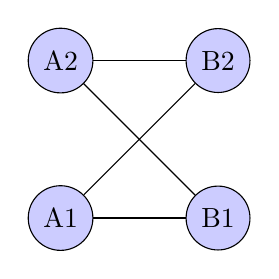
\begin{tikzpicture}
        % Vertices
        \node[circle, draw, fill=blue!20] (A1) at (0,0) {A1};
        \node[circle, draw, fill=blue!20] (A2) at (0,2) {A2};
        \node[circle, draw, fill=blue!20] (B1) at (2,0) {B1};
        \node[circle, draw, fill=blue!20] (B2) at (2,2) {B2};
        
        % Bipartite edges
        \draw (A1) -- (B1);
        \draw (A1) -- (B2);
        \draw (A2) -- (B1);
        \draw (A2) -- (B2);
    \end{tikzpicture}
    \caption{Bipartite graph example.}
    \label{fig:bipartite-graph}
\end{figure}
    
\end{itemize}

\subsection{Graph Representation}
Graphs can be represented in various ways, including:
\begin{itemize}
    \item \textbf{Adjacency Matrix} [\autoref{fig:adjacency-matrix}]: A square matrix $A$ of size $|V| \times |V|$ where $A_{ij} = 1$ if there is an edge between vertices $v_i$ and $v_j$, and $A_{ij} = 0$ otherwise.
    
   \begin{figure}[H]
    \centering
    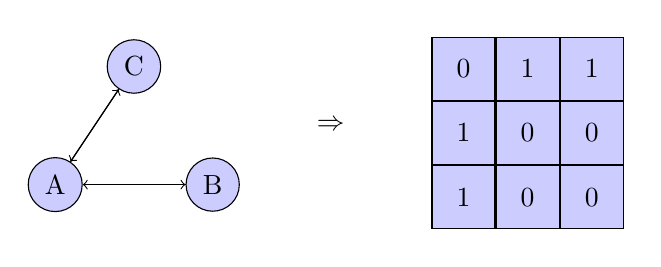
\begin{tikzpicture}
        % Define the vertices
        \node[circle, draw, fill=blue!20] (A) at (0,0) {A};
        \node[circle, draw, fill=blue!20] (B) at (2,0) {B};
        \node[circle, draw, fill=blue!20] (C) at (1,1.5) {C};
        
        % Define the edges
        \draw[->] (A) -- (B);
        \draw[->] (A) -- (C);
        \draw[->] (B) -- (A);
        \draw[->] (C) -- (A);
        
        % Adjacency matrix
        \node (RA) at (3.5,0.75) {$\Rightarrow$};

        \matrix (A) [nodes={draw, minimum size=0.8cm, fill=blue!20}, right=6cm, below=-2cm] {
            \node{0}; & \node{1}; & \node{1}; \\
            \node{1}; & \node{0}; & \node{0}; \\
            \node{1}; & \node{0}; & \node{0}; \\
        };
        
    \end{tikzpicture}
    \caption{Adjacency Matrix representation.}
    \label{fig:adjacency-matrix}
    \end{figure}
    
    \item \textbf{Adjacency List} [\autoref{fig:adjacency-list-undirected}]: An array of lists. The array contains a list for each vertex, and each list contains the vertices that are adjacent to the corresponding vertex.
    
\begin{figure}[H]
    \centering
    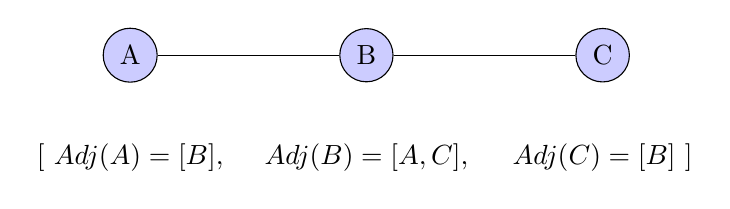
\begin{tikzpicture}
        % Define the vertices
        \node[circle, draw, fill=blue!20] (A) at (0,0) {A};
        \node[align=center, below] at (0, -1) {[ $Adj(A)=[B]$,};
        
        \node[circle, draw, fill=blue!20] (B) at (3,0) {B};
        \node[align=center, below] at (3, -1) {$Adj(B)=[A,C]$,};
        
        \node[circle, draw, fill=blue!20] (C) at (6,0) {C};
        \node[align=center, below] at (6, -1) {$Adj(C)=[B]$ ]};
        
        % Define the edges (undirected)
        \draw (A) -- (B);
        \draw (B) -- (C);
        
    \end{tikzpicture}
    \caption{Adjacency List representation for an undirected graph.}
    \label{fig:adjacency-list-undirected}
\end{figure}
    
\end{itemize}


\section{Graph Similarity Problem}

The \emph{graph similarity problem} involves determining the degree of similarity between two graphs. This problem has numerous applications in pattern recognition, computer vision, bioinformatics, and other fields. One common method to quantify graph similarity is through the \emph{graph edit distance} (GED).

\subsection{Graph Edit Distance (GED)}

The \emph{graph edit distance} between two graphs $G_1 = (V_1, E_1)$ and $G_2 = (V_2, E_2)$ is defined as the minimum cost required to transform $G_1$ into $G_2$ using a sequence of atomic operations. Formally, let $\Sigma$ be the set of all possible edit operations, and let $c: \Sigma \to \mathbb{R}^+$ be a cost function that assigns a positive real number to each operation. The GED is then given by:

\[
\text{GED}(G_1, G_2) = \min_{\sigma \in \Sigma^*} \sum_{o \in \sigma} c(o)
\]

where $\Sigma^*$ denotes the set of all finite sequences of operations from $\Sigma$, and $o$ represents an individual operation within a sequence $\sigma$.

The computation of GED is known to be \textbf{NP-HARD} \cite{NP_HARDNESS}, indicating that finding the exact minimum edit distance between two graphs is computationally intensive.

\subsection{Atomic Operations}

The basic atomic operations typically includes:

\begin{itemize}
    \item \textbf{Vertex Insertion}: Inserting a new vertex $v$ into the graph.
    \item \textbf{Vertex Deletion}: Deleting an existing vertex $v$ from the graph.
    \item \textbf{Edge Insertion}: Inserting a new edge $e = \{u, v\}$ into the graph.
    \item \textbf{Edge Deletion}: Deleting an existing edge $e = \{u, v\}$ from the graph.
\end{itemize}

To demonstrate the Graph Edit Distance (GED), consider pair of graphs represented in \autoref{fig:ged-graphs}:

\begin{figure}[H]
    \centering
    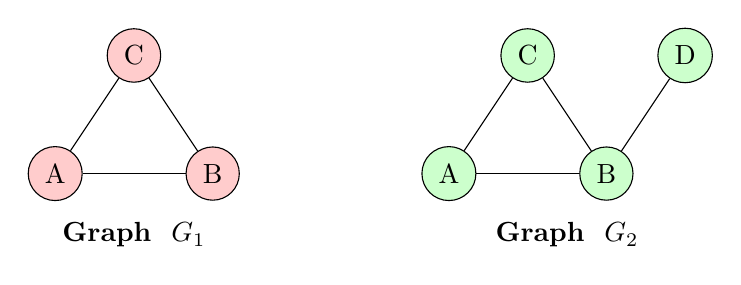
\begin{tikzpicture}
        % Define the vertices for G1
        \node[circle, draw, fill=red!20] (A1) at (0,0) {A};
        \node[circle, draw, fill=red!20] (B1) at (2,0) {B};
        \node[circle, draw, fill=red!20] (C1) at (1,1.5) {C};
        
        % Define the edges for G1
        \draw (A1) -- (B1);
        \draw (A1) -- (C1);
        \draw (B1) -- (C1);
        
        % Annotations for G1
        \node[align=center, below] at (1, -0.5) {\textbf{Graph } $G_1$};
        
        % Define the vertices for G2
        \node[circle, draw, fill=green!20] (A2) at (5,0) {A};
        \node[circle, draw, fill=green!20] (B2) at (7,0) {B};
        \node[circle, draw, fill=green!20] (C2) at (6,1.5) {C};
        \node[circle, draw, fill=green!20] (D2) at (8,1.5) {D};
        
        % Define the edges for G2
        \draw (A2) -- (B2);
        \draw (A2) -- (C2);
        \draw (B2) -- (C2);
        \draw (B2) -- (D2);
        
        % Annotations for G2
        \node[align=center, below] at (6.5, -0.5) {\textbf{Graph } $G_2$};
        
        
    \end{tikzpicture}
    \caption{Pair of graphs to demonstre Graph Edit Distance.}
    \label{fig:ged-graphs}
\end{figure}

In this example, graph $G_1$ has vertex set $V_1 = \{A, B, C\}$ and edge set $E_1 = \{\{A, B\}, \{A, C\}, \{B, C\}\}$, while graph $G_2$ has vertex set $V_2 = \{A, B, C, D\}$ and edge set $E_2 = \{\{A, B\}, \{A, C\}, \{B, C\}, \{B, D\}\}$. The transformation (which cost is lowest) from $G_1$ to $G_2$ involves: Inserting the vertex $D$ and Inserting the edge $\{B, D\}$. If we assign a cost of 1 to each operation the total cost (GED) is: $1+1=2$.

\section{Neural Networks}

\subsection{Neural Networks}

A \emph{neural network} is a computational model that is inspired by the way biological neural networks in the human brain process information. It consists of interconnected units called neurons that work together to solve specific problems. The basic building block of a neural network is the perceptron, which computes a weighted sum of its inputs and passes the result through an activation function.

\subsubsection{Basic Structure of a Neural Network}

A simple neural network [\autoref{fig:basic-nn}] consists of three types of layers:

\begin{itemize}
    \item \textbf{Input Layer}: The layer that receives the input data.
    \item \textbf{Hidden Layers}: One or more intermediate layers that process the inputs received from the input layer.
    \item \textbf{Output Layer}: The layer that produces the final output.
\end{itemize}

The following figure illustrates a basic neural network with one hidden layer:

\begin{figure}[H]
    \centering
    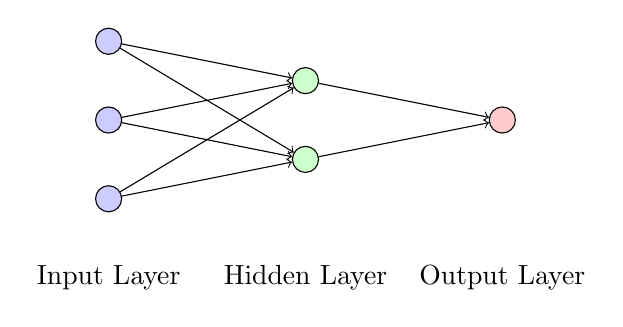
\begin{tikzpicture}
        % Define nodes
        \node[circle, draw, fill=blue!20] (I1) at (0,2) {};
        \node[circle, draw, fill=blue!20] (I2) at (0,1) {};
        \node[circle, draw, fill=blue!20] (I3) at (0,0) {};
        \node (I4) at (0,-1) {Input Layer};
        
        \node[circle, draw, fill=green!20] (H1) at (2.5,1.5) {};
        \node[circle, draw, fill=green!20] (H2) at (2.5,0.5) {};
        \node (H3) at (2.5,-1) {Hidden Layer};
        
        \node[circle, draw, fill=red!20] (O1) at (5,1) {};
        \node (O2) at (5,-1) {Output Layer};
        
        % Draw edges
        \foreach \i in {1,2,3}
            \foreach \j in {1,2}
                \draw[->] (I\i) -- (H\j);
                
        \foreach \i in {1,2}
            \draw[->] (H\i) -- (O1);
    \end{tikzpicture}
    \caption{A simple neural network with one hidden layer.}
    \label{fig:basic-nn}
\end{figure}
\subsection{Training Neural Networks}

Training a neural network involves adjusting the weights of the connections to minimize the error between the predicted output and the actual output. This is typically done using a method called \emph{backpropagation} along with an optimization algorithm like \emph{gradient descent}.

\subsubsection{Backpropagation}

Backpropagation [\autoref{fig:backpropagation}] is an algorithm used to compute the gradient of the loss function with respect to each weight by the chain rule, iterating backward from the last layer to the first layer.


\begin{figure}[H]
    \centering
    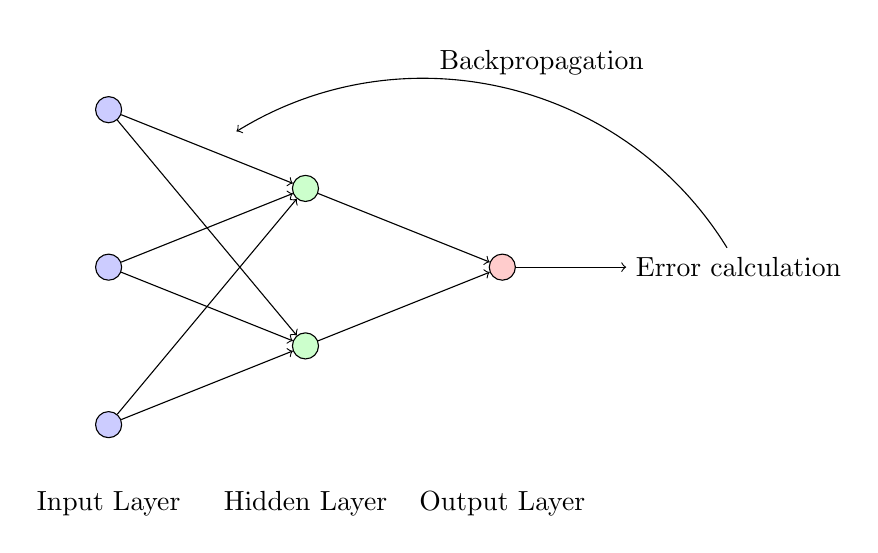
\begin{tikzpicture}
        % Define nodes
        \node[circle, draw, fill=blue!20] (I1) at (0,4) {};
        \node[circle, draw, fill=blue!20] (I2) at (0,2) {};
        \node[circle, draw, fill=blue!20] (I3) at (0,0) {};
        \node (I4) at (0,-1) {Input Layer};
        
        \node[circle, draw, fill=green!20] (H1) at (2.5,3) {};
        \node[circle, draw, fill=green!20] (H2) at (2.5,1) {};
        \node (H3) at (2.5,-1) {Hidden Layer};
        
        \node[circle, draw, fill=red!20] (O1) at (5,2) {};
        \node (O2) at (5,-1) {Output Layer};
        
        % Draw edges
        \foreach \i in {1,2,3}
            \foreach \j in {1,2}
                \draw[->] (I\i) -- (H\j);
                
        \foreach \i in {1,2}
            \draw[->] (H\i) -- (O1);
            
        
        \node (B1) at (8, 2) {Error calculation};
        \draw[->] (O1) -- (B1);
        
        \node (B2) at (1.5, 3.65) {};
        \draw[->] (B1) to [bend right=45] (B2);
        \node (B3) at (5.5, 4.6) {Backpropagation};
        
            
    \end{tikzpicture}
    \caption{A simple neural network with one hidden layer.}
    \label{fig:backpropagation}
\end{figure}


\subsubsection{Gradient Descent}

Gradient descent [\autoref{fig:grad-descent}] is an optimization algorithm used to minimize the loss function by iteratively moving towards the steepest descent, based on the computed gradients.

\begin{figure}[H]
\centering
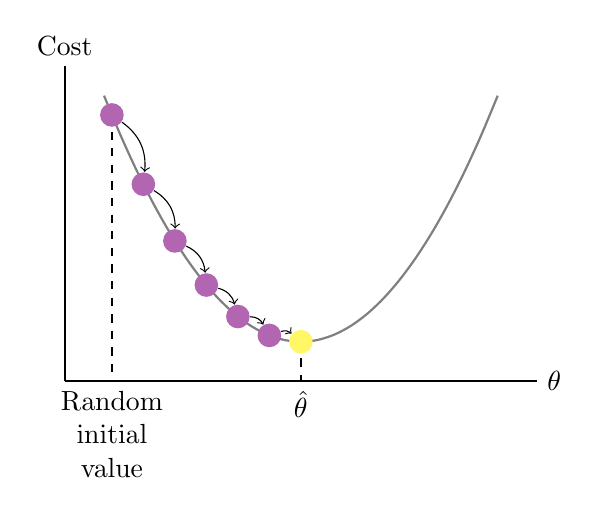
\begin{tikzpicture}[declare function={f(\x)=0.5*\x*\x-3*\x+5;}]
    \draw[thick](0,0)--(6,0) node[right]{$\theta$};
    \draw[thick,](0,0)--(0,4) node[above]{Cost};
    \draw[thick, dashed](0.6, {f(0.6)}) -- (0.6,0)
          node[below, text width=4em, align=center]{Random initial value};
    \draw[thick, dashed](3, {f(3)}) -- (3,0) node[below]{$\hat\theta$};
    \draw[domain=0.5:5.5, smooth, thick, gray] plot (\x, f(\x);
    \foreach \a [count=\c, remember=\c as \C] in {0.6, 1.0, ..., 2.6} {
      \node[circle, minimum size=3mm, inner sep=0pt, fill=violet!60] (\c) at (\a, {f(\a)}){};
      \ifnum\c>1
         \draw[->, bend left](\C) to (\c);
      \fi
    }
    \node[circle, minimum size=3mm, inner sep=0pt, fill=yellow!60] (Y) at (3, {f(3)}){}; 
    \draw[->, bend left](6) to (Y);
 \end{tikzpicture}
    \caption{Gradient descent method applied on a simple function.}
    \label{fig:grad-descent}
\end{figure}
\subsection{Advanced Topics in Neural Networks}

\subsubsection{Deep Neural Networks}

A \emph{deep neural network} (DNN) is an artificial neural network with multiple hidden layers between the input and output layers. DNNs can model complex patterns and relationships in data, making them powerful tools for tasks such as image and speech recognition.

\begin{figure}[H]
    \centering
    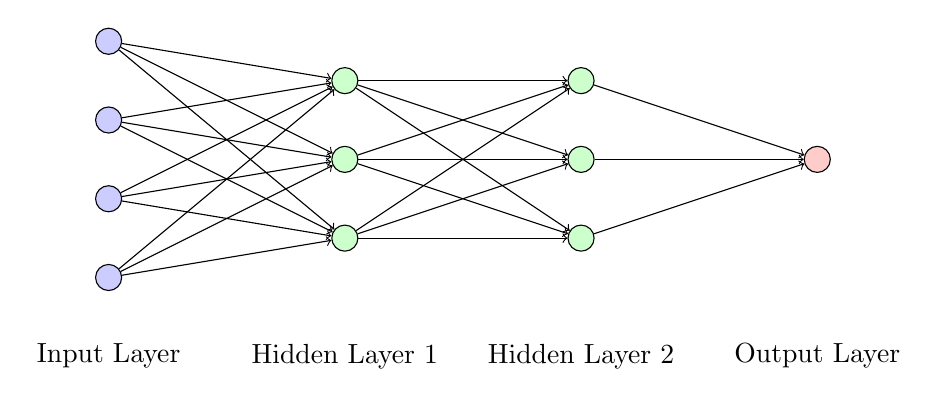
\begin{tikzpicture}
        % Define nodes
        \node[circle, draw, fill=blue!20] (I1) at (0,3) {};
        \node[circle, draw, fill=blue!20] (I2) at (0,2) {};
        \node[circle, draw, fill=blue!20] (I3) at (0,1) {};
        \node[circle, draw, fill=blue!20] (I4) at (0,0) {};
        \node (I5) at (0,-1) {Input Layer};
        
        \node[circle, draw, fill=green!20] (H11) at (3,2.5) {};
        \node[circle, draw, fill=green!20] (H12) at (3,1.5) {};
        \node[circle, draw, fill=green!20] (H13) at (3,0.5) {};
        \node (H14) at (3,-1) {Hidden Layer 1};
        
        \node[circle, draw, fill=green!20] (H21) at (6,2.5) {};
        \node[circle, draw, fill=green!20] (H22) at (6,1.5) {};
        \node[circle, draw, fill=green!20] (H23) at (6,0.5) {};
        \node (H24) at (6,-1) {Hidden Layer 2};
        
        \node[circle, draw, fill=red!20] (O1) at (9,1.5) {};
        \node (O2) at (9,-1) {Output Layer};
        
        % Draw edges
        \foreach \i in {1,2,3,4}
            \foreach \j in {1,2,3}
                \draw[->] (I\i) -- (H1\j);
                
        \foreach \i in {1,2,3}
            \foreach \j in {1,2,3}
                \draw[->] (H1\i) -- (H2\j);
                
        \foreach \i in {1,2,3}
            \draw[->] (H2\i) -- (O1);
    \end{tikzpicture}
    \caption{A Deep neural network with two hidden layers.}
    \label{fig:deep-nn}
\end{figure}

\subsubsection{Convolutional Neural Networks}

A \emph{convolutional neural network} (CNN) is a specialized type of neural network designed for processing structured grid data, like images. CNNs use convolutional layers that apply a series of filters to the input data to extract features.

\begin{figure}[H]
    \centering
    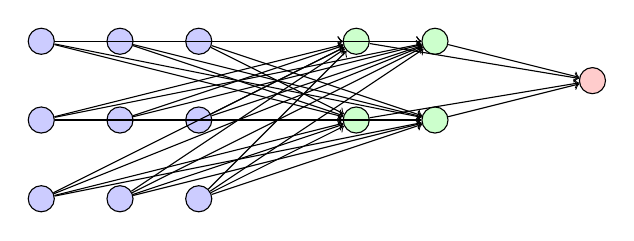
\begin{tikzpicture}
        % Input layer
        \foreach \i in {0,1,2}
            \foreach \j in {0,1,2} {
                \node[circle, draw, fill=blue!20] (I\i\j) at (\i,\j) {};
            }
        
        % Convolutional layer
        \foreach \i in {0,1}
            \foreach \j in {0,1} {
                \node[circle, draw, fill=green!20] (C\i\j) at (\i+4,\j+1) {};
            }
        
        % Fully connected layer
        \node[circle, draw, fill=red!20] (FC) at (7,1.5) {};
        
        % Connections
        \foreach \i in {0,1,2}
            \foreach \j in {0,1,2} {
                \foreach \m in {0,1}
                    \foreach \n in {0,1} {
                        \draw[->] (I\i\j) -- (C\m\n);
                    }
            }
        \foreach \i in {0,1}
            \foreach \j in {0,1} {
                \draw[->] (C\i\j) -- (FC);
            }
    \end{tikzpicture}
    \caption{A simple convolutional neural network architecture.}
    \label{fig:cnn}
\end{figure}


\subsubsection{Recurrent Neural Networks}

A \emph{recurrent neural network} (RNN) is a type of neural network that is well-suited for sequential data, such as time series or natural language. RNNs have connections that form directed cycles, allowing information to persist.

\begin{figure}[H]
    \centering
    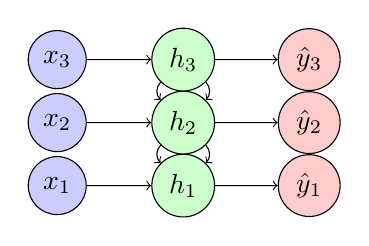
\begin{tikzpicture}[scale=0.8]
        % Time steps
        \foreach \t in {1,2,3} {
            % Input
            \node[circle, draw, fill=blue!20] (X\t) at (0,\t) {$x_\t$};
            
            % Hidden state
            \node[circle, draw, fill=green!20] (H\t) at (2,\t) {$h_\t$};
            
            % Output
            \node[circle, draw, fill=red!20] (Y\t) at (4,\t) {$\hat{y}_\t$};
            
            % Connections
            \draw[->] (X\t) -- (H\t);
            \draw[->] (H\t) -- (Y\t);
            
            % Recurrent connections
            \ifnum\t>1
                \draw[->] (H\t) to[bend left=45] (H\the\numexpr\t-1\relax);
                \draw[->] (H\t) to[bend right=45] (H\the\numexpr\t-1\relax);
            \fi
        }
    \end{tikzpicture}
    \caption{Recurrent Neural Network (RNN) unrolled through time.}
    \label{fig:rnn}
\end{figure}



\subsection{Graph Neural Networks and Attention Mechanisms}

\subsubsection{Graph Neural Networks}

A \emph{graph neural network} (GNN) is a type of neural network designed to handle graph-structured data. GNNs generalize neural networks to work directly on the graph domain by incorporating the graph's structure into the learning process. Nodes in a GNN aggregate feature information from their neighbors through multiple layers, enabling the network to capture the dependencies and relationships inherent in the graph.

\begin{figure}[H]
    \centering
    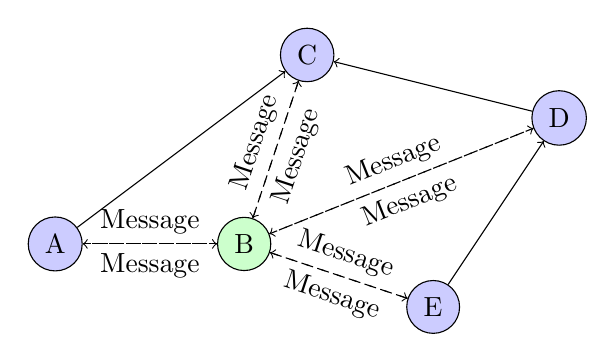
\begin{tikzpicture}[scale=0.8]
        % Nodes
        \node[circle, draw, fill=blue!20] (A) at (0,0) {A};
        \node[circle, draw, fill=green!20] (B) at (3,0) {B};
        \node[circle, draw, fill=blue!20] (C) at (4,3) {C};
        \node[circle, draw, fill=blue!20] (D) at (8,2) {D};
        \node[circle, draw, fill=blue!20] (E) at (6,-1) {E};
        
        % Edges
        \draw[->] (A) -- (C);
        \draw[->] (D) -- (C);
        \draw[->] (E) -- (D);
        
        % Message passing
        \draw[->, dashed] (A) -- (B) node[midway, above, sloped] {Message};
        \draw[->, dashed] (B) -- (A) node[midway, below, sloped] {Message};
        \draw[->, dashed] (C) -- (B) node[midway, above, sloped] {Message};
        \draw[->, dashed] (B) -- (C) node[midway, below, sloped] {Message};
        \draw[->, dashed] (B) -- (D) node[midway, above, sloped] {Message};
        \draw[->, dashed] (D) -- (B) node[midway, below, sloped] {Message};
        \draw[->, dashed] (B) -- (E) node[midway, below, sloped] {Message};
        \draw[->, dashed] (E) -- (B) node[midway, above, sloped] {Message};
    \end{tikzpicture}
    \caption{Message passing between node B and its neighbors in a GNN.}
    \label{fig:gnn}
\end{figure}




\subsubsection{Attention Mechanisms}

Attention mechanisms are techniques used to enhance the performance of neural networks by dynamically focusing on relevant parts of the input data while processing. The most famous use of attention mechanisms is in the \emph{Transformer} model, which has revolutionized natural language processing tasks. The attention mechanism computes a weighted sum of values, where the weights are derived from the compatibility of the query with the corresponding keys, allowing the model to selectively focus on important parts of the input.

The combination of GNNs and attention mechanisms has shown significant promise in various applications, such as molecular property prediction, social network analysis, and more.

\begin{figure}[H]
    \centering
    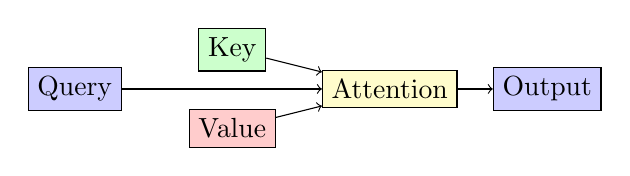
\begin{tikzpicture}
        % Define nodes
        \node[rectangle, draw, fill=blue!20] (Q) at (0,1) {Query};
        \node[rectangle, draw, fill=green!20] (K) at (2,1.5) {Key};
        \node[rectangle, draw, fill=red!20] (V) at (2,0.5) {Value};
        
        % Attention weights
        \node[rectangle, draw, fill=yellow!20] (A) at (4,1) {Attention};
        
        % Output
        \node[rectangle, draw, fill=blue!20] (O) at (6,1) {Output};
        
        % Connections
        \draw[->] (Q) -- (A);
        \draw[->] (K) -- (A);
        \draw[->] (V) -- (A);
        \draw[->] (A) -- (O);
    \end{tikzpicture}
    \caption{Attention mechanism in neural networks.}
    \label{fig:attention}
\end{figure}



\section{SimGNN}
\section{Bottleneck Loading GPU Problem}
\section{Dataset Generation}
\section{State of the Art Review}


\bibliographystyle{plain}
\bibliography{References}


\end{document}
